


\section{Evaluation protocols}
\label{sec_protocols}
In this section, we present 3 protocols which can be used to verify the
hypotheses detailed in \autoref{Hypotheses}. One can directly use these
algorithms on the ensemble dataset. It corresponds to $(i)$ the separation of
the schemes and the independence of the orders, $(ii)$ the unique behavior of
the HLL solver and $(iii)$ similarities in class of solvers.


\subsection{Persistence curves}
\label{sec_persistence}
With this protocol (illustrated on toy examples, \autoref{fig_gaussian_curve}), we want to validate hypothesis H1 (\autoref{Hypotheses}) to discriminate the interpolation schemes TENO and WENO-Z regarding the differences in the enstrophy field. With this protocol, we also want to validate hypothesis H2 (\autoref{Hypotheses}) to confirm the independence of the orders \cite{san2015evaluation}. To better characterize the vortices influencing the turbulence, we use persistence curves (\autoref{sec_topology}). These curves will
allow us to threshold the structures (the eddies) at different scales and
thus to easily compare the number of small (\autoref{fig_gaussian_curve}a) and large (\autoref{fig_gaussian_curve}b) eddies using the integral of the persistence curve.

For the differentiation of the schemes, we take 5 simulation configurations where the physical time ($t_0,t_1,t_2$), the resolution ($256\times 256$, $512\times 512$, $ 1024\times 1024$) and the order (5,7) are fixed per sample (\autoref{tab_parameters}). The variation is the interpolation scheme (TENO, WENO-Z). For the order independence, 5 configurations are also chosen by fixing the physical time ($t_0,t_1,t_2$), the resolution ($256\times 256$, $512\times 512$, $ 1024\times 1024$), the scheme (TENO or WENO-Z). The variation is done on the order (5,7). Besides different input variations,
% to build the configurations,
this protocol is the same for testing H1 and H2.

The persistence curves are generated for all the samples. Then, we average the 5 persistence curves (one per solver) to obtain 2 average persistence curves with respect to the variable parameters (schemes or orders). Finally, we compute the difference of the integrals between the two averaged curves (grey area on \autoref{fig_gaussian_curve}). The small values on the curves under a persistence of $10^{-6}$ correspond to numerical noise coming from the different simulation steps. They are removed from the computation of the integral with a threshold at $10^{-6}$(\autoref{fig_gaussian_curve}.a). The integral curve difference corresponds to our metric allowing to precisely describe the similarity in the topology of the critical points. Bigger is the integral, the more different the topology of the flow is. Thus, to verify hypothesis H1 related to the scheme, we want the difference of the integrals to be high. To verify hypothesis H2 related to the orders, we want the difference of the integrals to be close to zero.


\begin{figure}
 \centering
 \vspace{-1ex}
 
\includegraphics[width=\figureShrink\linewidth]{chapter4_topology_data_analysis/pictures/gaussian_distance_to_the_rest.jpg}
 \mycaption{
 Wasserstein distance matrix for five inputs $S_1$, $S_2$, $S_3$,$S_4$, $S_5$
 generated respectively with two, five, four and three Gaussians
%  functions
 with varying noise.
% different noise levels.
The sum of each
matrix line
% line of the matrix
is
% computed and
normalized with respect to the scalar-field that maximizes the distances, here
$S_1$. We see that $S_1$ with only two Gaussians is very far from the other
datasets.}
 \label{gaussian_distance}
\end{figure}
\begin{figure}
\vspace{-1ex}
 \centering % avoid the use of \begin{center}...\end{center} and use \centering
 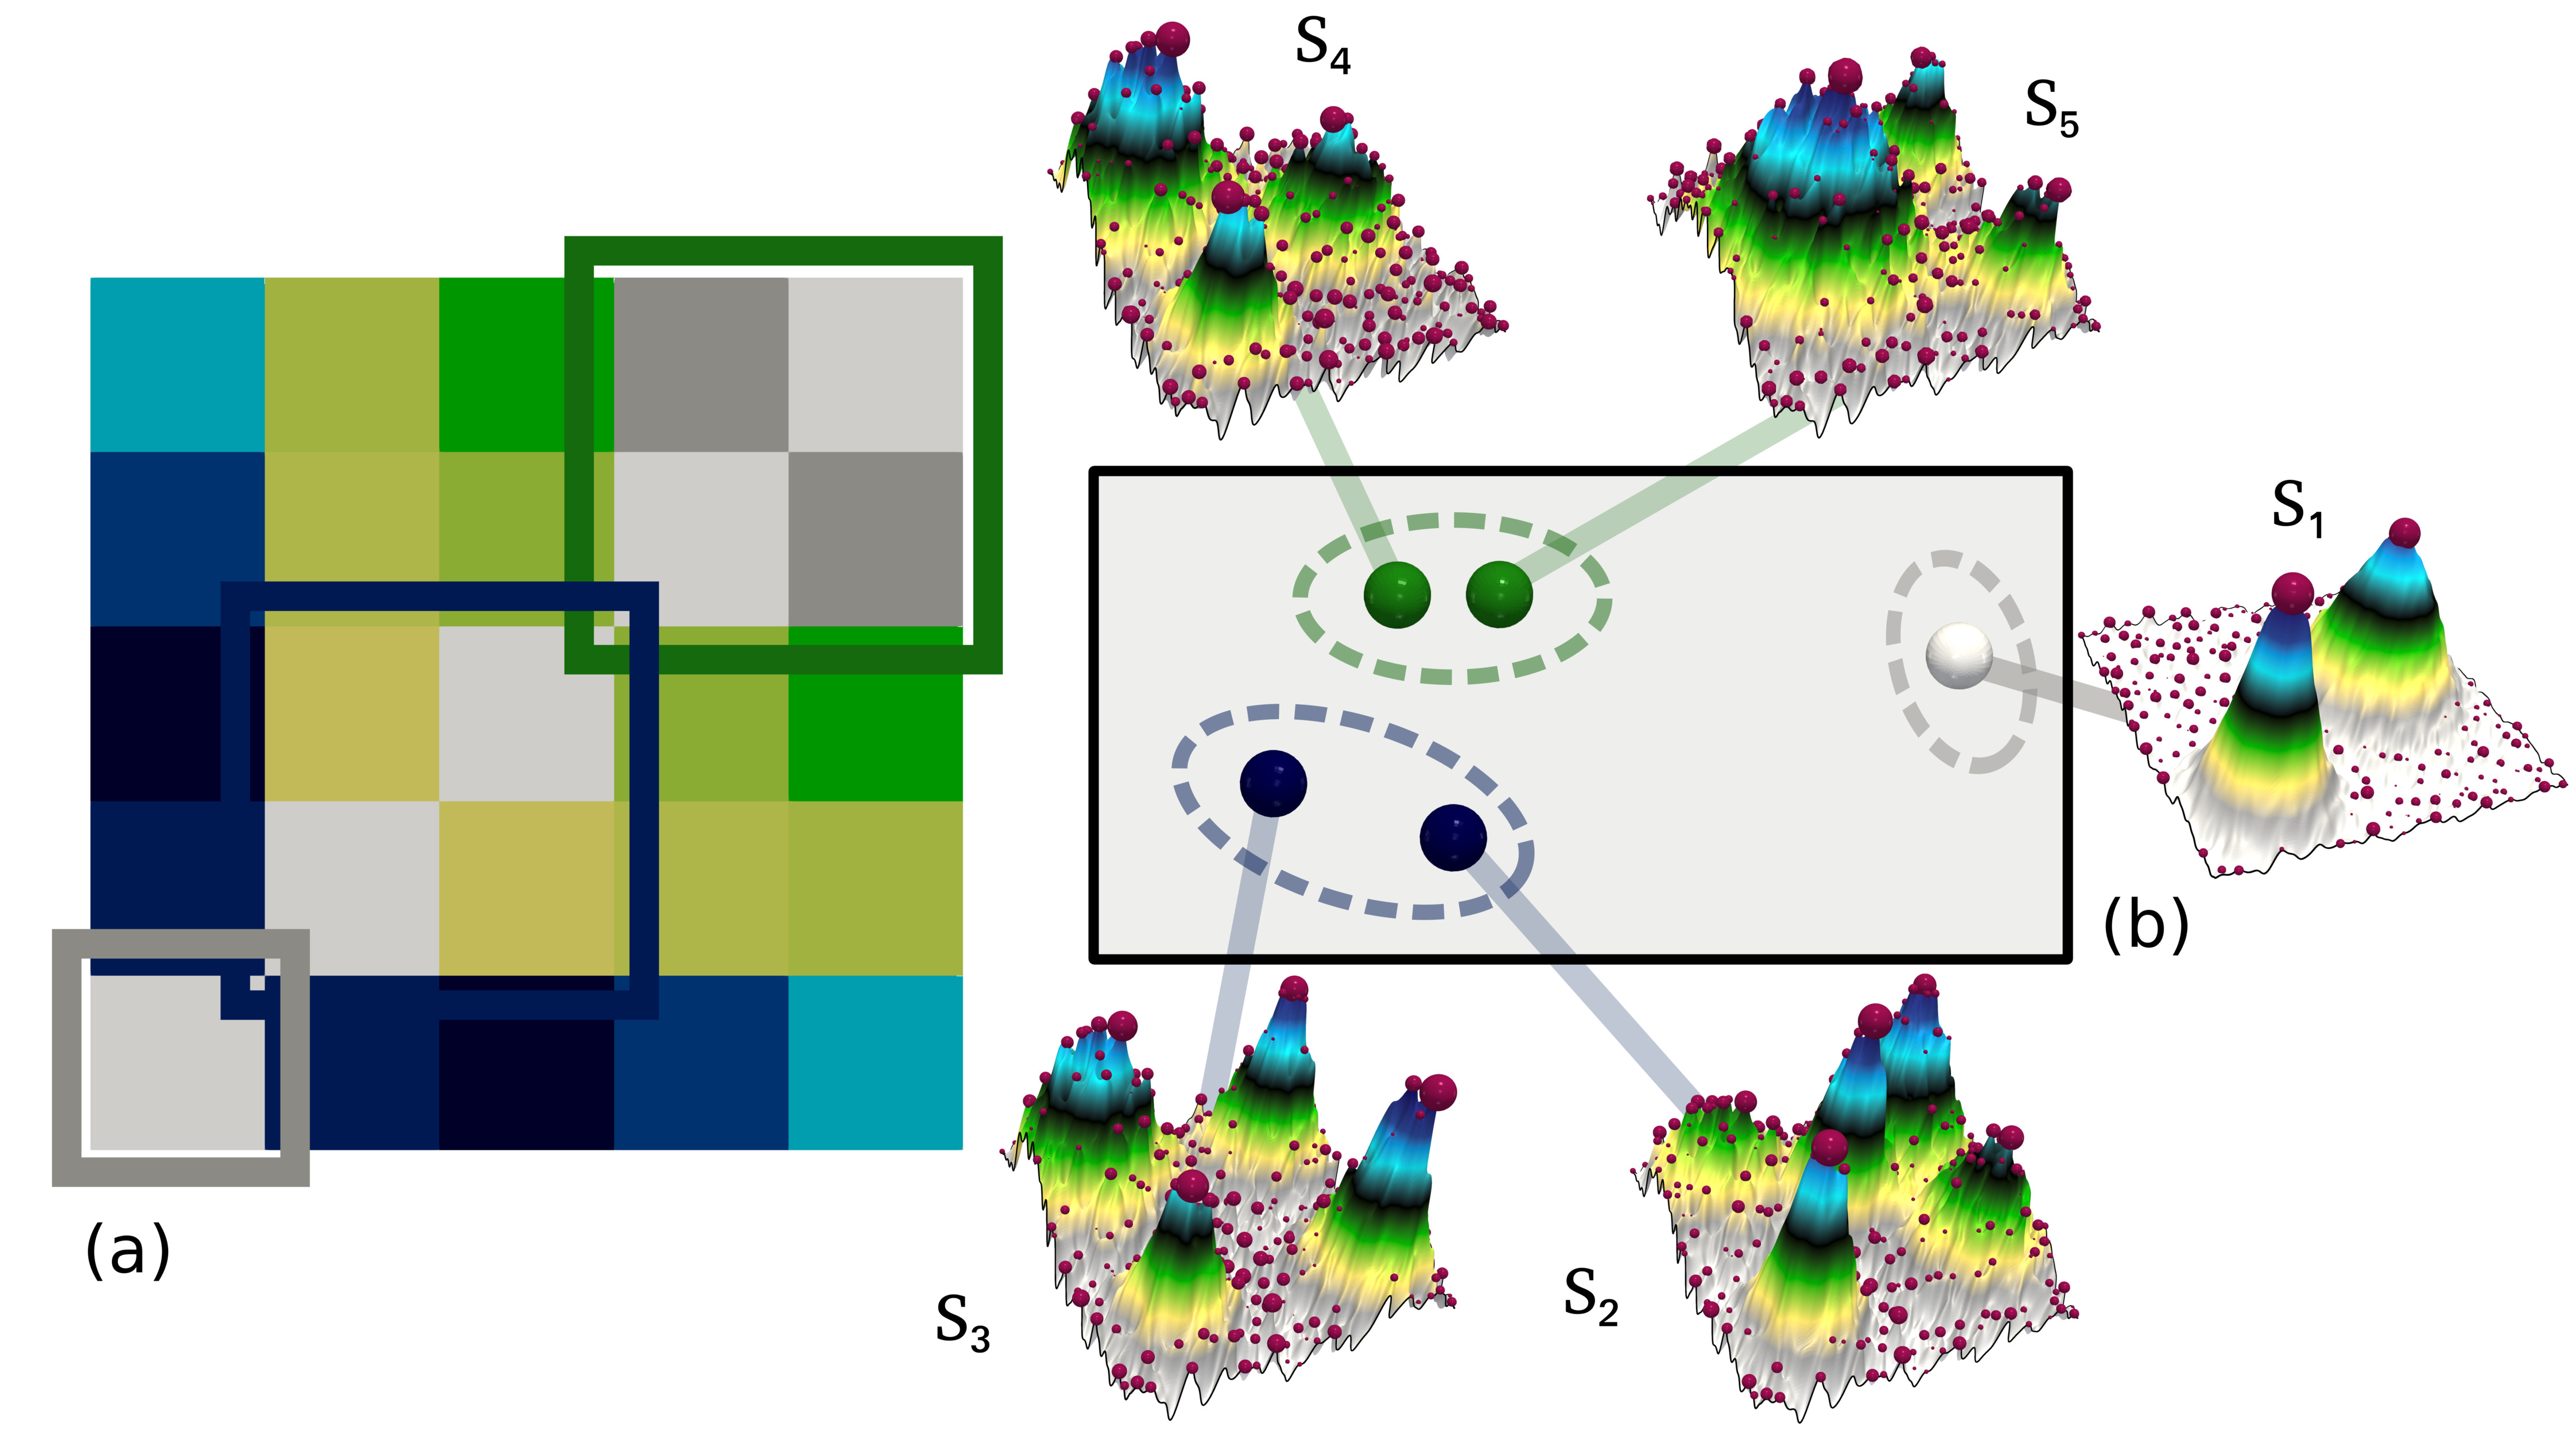
\includegraphics[width=\figureShrink\linewidth]{chapter4_topology_data_analysis/pictures/gaussian_cluster.jpg}
 \mycaption{
 Wasserstein distance matrix for five inputs $S_1$, $S_2$, $S_3$, $S_4$, $S_5$ generated respectively with two, five, for and three Gaussian
functions with different noise levels. Point cloud of the inputs in the Wasserstein distance space colored according to the clusters obtained with the k-means clustering method. We can see that each terrain in a cluster has the same number of Gaussian and level of noise.}
 \label{gaussian_cluster}
\end{figure}
\begin{figure*}
 \centering % avoid the use of \begin{center}...\end{center} and use \centering
 
\includegraphics[width=\figureShrink\linewidth]{chapter4_topology_data_analysis/pictures/KHI_courbes.jpg}
 \mycaption{
Schemes (left) and order (right) studies.
% , left orders study.
Average
persistence curves for 5 configurations with variations of : a (WENO-Z,5), c
(WENO-Z, 7), f (WENO-Z, 5), h (TENO,5). (b,g) persistence curves at $t_0$ (top),
$t_1$ (middle), $t_2$ (bottom).
 Vertical lines on the curves correspond to critical points of small (left) and
high (right) persistence.
% critical points (left) and high persistence (right).
(d,e) Integral differences (grey area) between average persistence curves for
all variations.}
\vspace{2ex}
 \label{curv}
\end{figure*}

\begin{figure*}
 \centering
 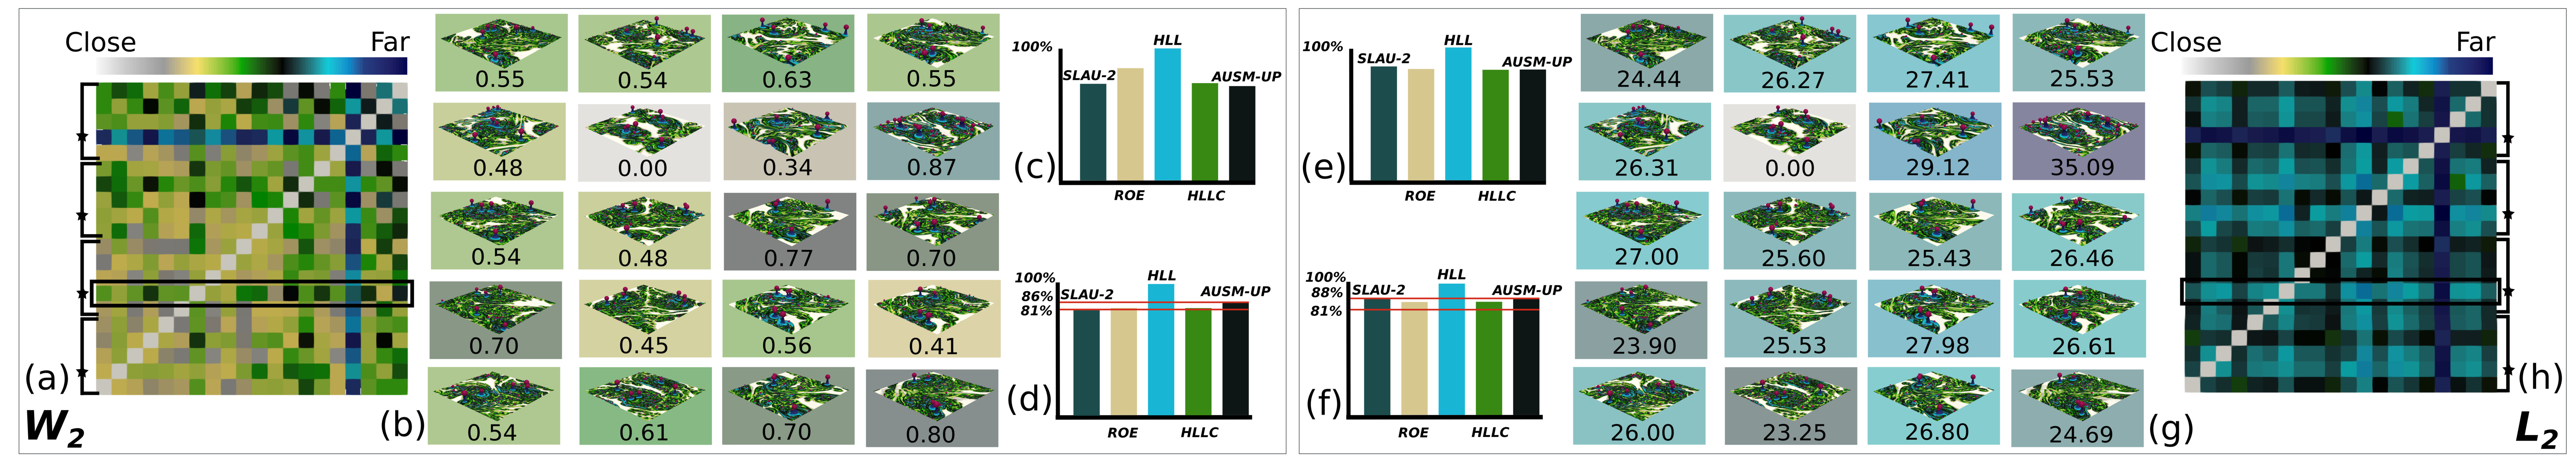
\includegraphics[width=\figureShrink\linewidth]{chapter4_topology_data_analysis/pictures/KHI_distance_to_the_rest.jpg}
 \mycaption{Comparison between the $\wasserstein{2}$ metric (left) and the standard $L_2$-metric (right) for isolating the HLL solver.
 (a,h) Distance matrix for 20 configurations at $t_2$ at $512 \times 512$. Black frames represent the distance between the TENO 7$_{th}$ order with the HLL (matrix lines marked by $\star$) and the other configurations (b,g). Histograms (c,e) are respectively the percentage average of the sum distance matrix of (a,h). Histograms (d,f) are respectively the percentage of the sum distance for all variations.}
 \label{fig_KHIdistance}
\end{figure*}


\subsection{Outlier distance profile}
\label{sec_outlier}
With this protocol (illustrated on toy examples,
\autoref{gaussian_distance}), we want to validate hypothesis H3 (\autoref{Hypotheses}), which means that for all the simulation configurations the HLL solver will be very different from other solvers to describe the Kelvin-Helmholtz instabilities. For this protocol, we take 5 simulation configurations where we fix the reconstruction (TENO or WENO-Z), the physical time ($t_0$, $t_1$, $t_2$), the mesh ($256\times 256, 512\times 512, 1024\times 1024$), the order (5 or 7) and we vary the solvers. The 5 different computations describing the same turbulent flow obtained with the solvers (HLL, SLAU2, AUSM$^+$-UP, HLLC and Roe) are analyzed regarding to the enstrophy.

A distance is used to compare the topology of the enstrophy. Many methods can be used to compute such a distance but in this protocol we focus on 2 metrics: the $L_2$-norm distance directly on the values of the enstrophy and the Wasserstein distance on the persistence diagrams. One can inject other distances if needed. For the Wasserstein, the saddle-maximum persistence diagram is computed on each result. Then, they are grouped in a unique dataset to compute a persistence diagram distance matrix (\autoref{gaussian_distance}). For the $L_2$-norm, a distance matrix  is also created where a line corresponds to the distance in the enstrophy field from one solver to the others.





Thus, the sum of the distances from one solver to the others is computed by
summing the distances on one line of the matrix. The total distance of one 
solver to the others, for all configurations, is simply the sum of all these sum 
distances for every line of the matrix which correspond to the same solver. We 
finally obtain one global distance per solver for all configurations. Finally 
the difference between the distance of the HLL and the distance of the maximizer 
(the second value if HLL is the maximum) gives a separation score. If the
difference is positive, then hypothesis H3 is verified whereas it is not if 
negative, because it means that another solver generates a flow topologically 
more different than the HLL. 
With this protocol, best separations are obtained for high absolute values.
% of 
% the score.

% the higher is the absolute value of the score, the 
% better the separation is.
% with this protocol.



\subsection{Unsupervised classification}
\label{sec_unsupervised}


With the last protocol (illustrated on toy examples in \autoref{gaussian_cluster}),
we want to validate hypotheses H4 and H5 (\autoref{Hypotheses}). We want to verify that the
simulations with the Roe and HLLC solvers are topologically close (hypothesis H4) and the
simulations with the AUSM$^+$-UP and SLAU2 solvers are topologically close (hypothesis H5). To do so, three clustering methods will be used based on Wasserstein distances and the L$_2$- norm(\autoref{sec_topology}).

For the first two clustering methods, we start by computing distance matrix with the protocol of the outlier distance profile \autoref{sec_outlier} using successively the Wasserstein distance and $L_2$-norm matrices (\autoref{gaussian_cluster}a). We apply a dimension reduction to project the distances of the matrix according to 2 components (\autoref{sec_topology}). This projection is used to generate clusters of the matrices with a k-means algorithm (\autoref{sec_topology}) as illustrated on \autoref{gaussian_cluster}b. The third clustering method uses directly the persistence diagrams(\autoref{sec_topology}) without using the distance matrix. All the persistence diagrams are merge into a single dataset to compute the Wasserstein distances between each diagram. The barycenter of persistence diagram is then used to directly compute a cluster, without dimension reduction, in the Wasserstein metric space \cite{vidal_vis19} with the ${W_2}$ distance. Then a k-means algorithm (\autoref{sec_topology}) is applied. 

With these three classification methods, we obtain different associations of our configurations. Each association is going to be scored with a measure of similarities between the clusters regarding to a reference cluster using the Rand Index \cite{rand1971objective}. This Rand index has a value between 0 and 1, with 0 indicating that two clusters do not agree on any pair of points and 1 indicating that the data clusters are exactly the same. Based on the properties of the solvers used in the simulation code HYPERION and detailed in \autoref{sec_solvers}, we define our reference cluster such that the first partition contains the AUSM$^+$-UP and SLAU2 solvers, the second partition the HLLC and Roe solvers and the third partition the HLL solver. The Rand Index is computed for each configuration and averaged per clustering method.
This
% metric
enables the
% precise
ranking of
% allows us to precisely rank
the different solver
behaviors.
% of our solvers.
If the average Rand Index score is close to 1 then both hypotheses H4, showing similarity between the AUSM$^+$-UP and SLAU2 solvers and H5, showing the isolation of the HLL solver, are verified.










